\documentclass[preprint]{aastex62}

% \usepackage{minted}
\usepackage{listings}
\usepackage{courier}

\definecolor{bcolor}{RGB}{0, 51, 153}
\definecolor{gcolor}{RGB}{51, 153, 51}

\shorttitle{photon counting \& detectors}
\shortauthors{j. birky}

\begin{document}

\title{\sc Lab 1: Photon Counting \& Detectors}
\author{Jessica Birky, Julian Beaz-Gonzalez, Russell Van-Linge}

\correspondingauthor{Jessica Birky (A13002163)}
\email{jbirky@ucsd.edu}

\begin{abstract}
This example manuscript is intended to serve as a tutorial and template for
authors to use when writing their own AAS Journal articles. The manuscript
includes a history of and documents the new features in the
previous versions as well as the new features in version 6.2. This
manuscript includes many figure and table examples to illustrate these new
features.  Information on features not explicitly mentioned in the article
can be viewed in the manuscript comments or more extensive online
documentation. Authors are welcome replace the text, tables, figures, and
bibliography with their own and submit the resulting manuscript to the AAS
Journals peer review system.  The first lesson in the tutorial is to remind
authors that the AAS Journals, the Astrophysical Journal (ApJ), the
Astrophysical Journal Letters (ApJL), and Astronomical Journal (AJ), all
have a 250 word limit for the abstract.  If you exceed this length the
Editorial office will ask you to shorten it.

\end{abstract}
\bigskip

\section{Introduction} 
In order to understand the. Advancements in technology in the 20th century has now made it possible to observe electromagnetic radiation from the scales of $10^{-12}-10^3$m (as short as gamma rays to as long as radio waves). Understanding how detectors work, the statistics of light collection, as well as the limitations of the instrument and sources of contaminations are a fundamental first steps before performing any scientific analysis of light with an instrument.

CCDs, the photoelectric effect

Types of noise we want to quantify

% ==================================
\section{Observations}
Nickel telescope, what are bias and flat frames


% ==================================
\section{Data Reduction \& Methods}
\subsection{Theoretical Distribution of Light}
Before we can characterize our observations, it is important to first determine what we expect our data will look like. That is, we are measuring the number of photons hitting a detector over a fixed amount of time, what do we predict will be the number of photons that will hit each pixel in that tme interval? Let's assume that on average $\mu$ photons will hit a pixel over fixed time interval $t$. Now consider dividing that time interval into $n$ increments: the probability that a $n$ photons arrive to the detector is approximately Binomial. Now in the limit that $n\rightarrow\infty$, we arrive at the Poisson distribution:
\begin{equation}
P(x;\mu) = \frac{\mu^x}{x!}e^{-\mu}
\end{equation}
which we interpret as the probability that x photons will arrive to a detector pixel in time interval $t$, given that $\mu$ photons arrive in that interval on average. The expected mean and variation for this distribution being $\langle x \rangle = \mu$ and $\langle \sigma^2 \rangle = \mu$. Under the conditions that the number of observations is much smaller than the mean of the distribution ($n << \mu$), and 

In practice, the Poisson distribution is unstable to compute for large values of x because the term $x!$ becomes too large for the memory of the computer to handle. In order to try to reduce the memory load for large values of x, we approximate the $x!$ term using the Sterling approximation:
\begin{equation}
n! \sim \sqrt{2\pi n}\left(\frac{n}{e} \right)^n
\end{equation}
the code for the Poisson distribution is implemented in lines $7-9$ of Appendix \ref{code:stats}.

However when the conditions for the Poisson distribution are not met very well, the Gaussian distribution is a good approximation:
\begin{equation}
P(x; \mu, \sigma) = \frac{1}{\sqrt{2\pi}} e^{-\frac{(x-\mu)^2}{2\sigma^2}}
\end{equation}
the code for the Gaussian distribution is implemented in lines $11-13$ of Appendix \ref{code:stats}.

\subsection{Data Manipulation}
Procedure to combine frames and subtract bias, point to code

\subsection{Types of Detector Noise}
How to calculate the readnoise, other noise, error propagation

% ==================================
\section{Data Analysis \& Modeling}
\subsection{Bias Frames}

\begin{figure}[ht]
\plotone{plots/exposure0.png}
\caption{Combined bias frames.} \label{fig:bias}
\end{figure}

\subsection{Combined Images \& Histograms}
The figures in \ref{fig:flats1} and \ref{fig:flats2} show the bias-subtracted, combined histograms and images for each of the eight different exposure times (3, 6, 12, 24, 48, 96, 192, 384, and 768 seconds). The left side of each panel shows the histogram of the number of detector counts in analog to digital units (ADU), normalized such that the sum of all of the bins is one (plotted in black). The solid blue vertical line marks the mean of the data, and the dashed blue line marks the median, indicating which distrubtions are skewed by outlying points (where the mean is far from the median): in the combined bias frame the mean is skewed higher than the center of the distribution, and for all of the other exposures the mean is skewed lower than the center. The two shades of green mark $\pm1$ and $\pm2$ standard deviations above and below the mean. For all distributions, the $\pm1\sigma$ lines lie far outside of the bulk of the distribution around the median, which indicates again that there are many outlying the part of the distribution shown. Finally, the distribution in red shows the expected Poisson distribution, as a function of the mean of the data ($\bar{x}$), with a one standard deviation range also shaded in red (where the expected standard deviation for the Poisson is $\sigma=\sqrt{\bar{x}}$).  

The right side of each panel shows the 2D images. In order to visualize the detector counts per pixel, we must map the number of counts to an RGB color value, which we use the matplolib 'gray' colormap for. To emphasize the features in the data, we choose the min an max values of the colormap to be the 10th and 90th percentile counts of the data.


\begin{figure}[ht]
\plotone{plots/exposure3.png}
\plotone{plots/exposure6.png}
\plotone{plots/exposure12.png}
\plotone{plots/exposure48.png}
\caption{Combined, bias-subtracted, flat frame histograms and images for varying exposure times (0, 3, 6, and 12 sec). \label{fig:flats1}}
\end{figure}
\begin{figure}[ht]
\plotone{plots/exposure96.png}
\plotone{plots/exposure192.png}
\plotone{plots/exposure384.png}
\plotone{plots/exposure768.png}
\caption{Combined, bias-subtracted, flat frame histograms and images for varying exposure times (96, 192, 384, and 768 sec). \label{fig:flats2}}
\end{figure}

\subsection{Mean of the Mean \& Standard Deviation of the Mean}
Describe computation, show plots

\subsection{Quatifying Detector Noise}
Calculate readnoise n stuff

\begin{figure}[ht]
\begin{center}
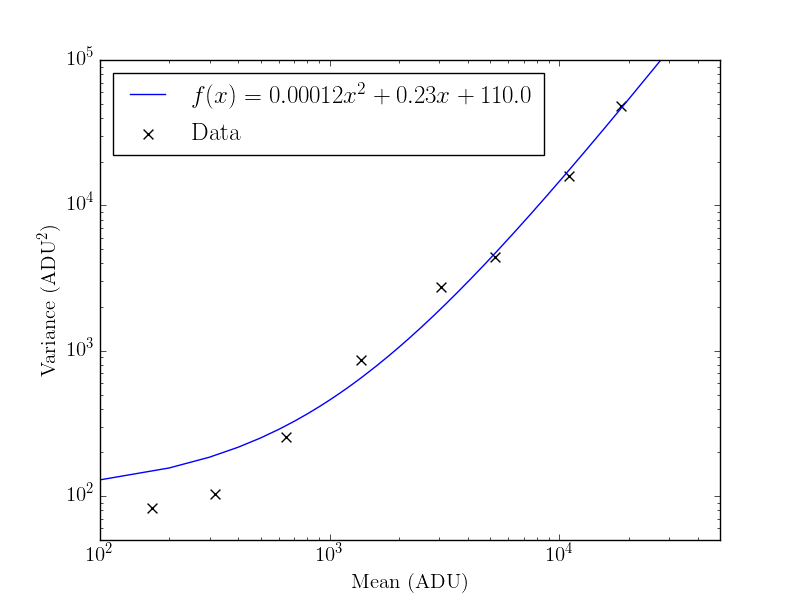
\includegraphics[width=.48\linewidth]{plots/mean_vs_variance.png}
\caption{Mean vs. variance for all bias-subtracted exposures, fitted to a second-order polynomial.} \label{fig:mean_var}
\end{center}
\end{figure}

% ==================================
\section{Discussion}
\subsection{Poisson Comparisons}
Looking at Figures \ref{fig:flats1} and \ref{fig:flats2}, we find that the detector count distribution is close to a Poisson distribution for low exposure times, but for larger exposure times it increasingly diverges with a much larger standard deviations than expected (as summarized by Figure \ref{fig:mean_var}). We also see that low exposure times (3, 6, and 12 sec) have a single peak in the distribution around the mean, however at 48 sec the distribution becomes bimodal, and for high exposure times (96, 192, 384, and 768 sec) the distribution develops three separate peaks. Comparing these histograms to the corresponding images at the right, we can see the regions on the detector which correspond to the different peaks: the dark edges make up roughly the bottom third of the distribution, and the bright center making up the higher thrid of the distribution. If the distribution was Poissonian for each pixel, we would expect the signal to vary uniformly across the detector, but instead there is obvious contamination at different spatial regions.

\subsection{Sources of Noise \& Systematic Effects}
Variations in the quantum efficiency of each pixel.
Dust particles on the lens scatter and absorb light unevenly at different points on the detector.

Checked for systematics due to temperature variation that could maybe be responsible for dark current: found temperature to vary only within 4C (Figure \ref{fig:temp}). Checked for systematic differences in different datasets. 

\begin{figure}[ht]
\begin{center}
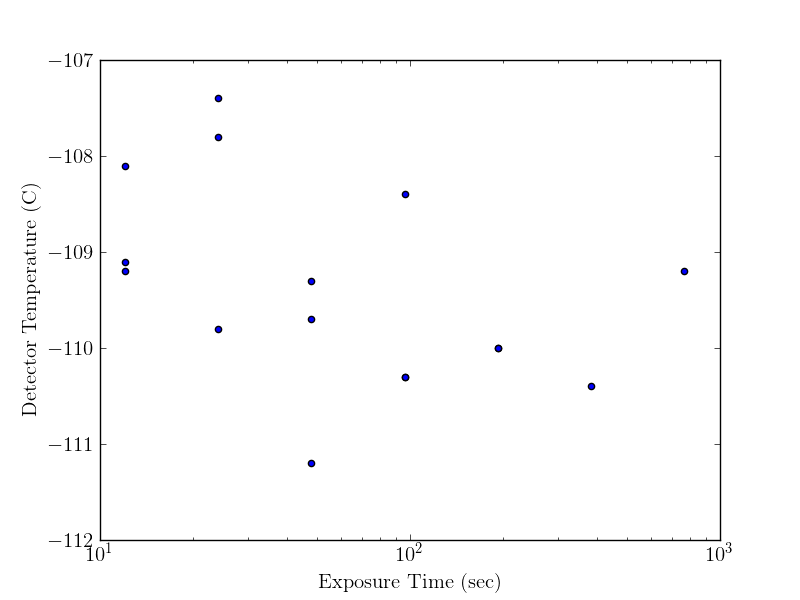
\includegraphics[width=.48\linewidth]{plots/exposure_temp.png}
\caption{Temperature of the CCD detector for different exposure frames does not vary more than about 4C.} \label{fig:temp}
\end{center}
\end{figure}

% ==================================
\section{Conclusion}

% ==================================
\section{Author Contributions}

This project was done in collaboration with Julian Beas-Gonzalez and Russell Van-Linge (Group E), using data collected by Group B. Russell wrote code for fitting Poisson and Gaussian distribtions and computing MOM/SDOM, Julian wrote code for histograms and computing MOM/SDOM, and I wrote code for combining frames/bias subtracting images, plotting histograms/images and slicing images (except for a few snippets for making histograms and reading fits files from the class notes). We met several times outside of class to compare results, fix issues, and combine our code together, which can be found on github: \href{https://github.com/jbirky/photonCounting}{https://github.com/jbirky/photonCounting}.

% ==================================
\section{Appendix}

\subsection{Statistics}
Mean and variance for a set of data points $x={x_1, ...,x_N}$:
\begin{equation}
	\bar{x} = \frac{1}{N} \sum^N_{i=1} x_i  
\end{equation}
\begin{equation}
	s^2 = \frac{1}{N-1} \sum^N_{i=1} (x_i - \bar{x})^2
\end{equation}

\subsection{Code}

\lstset{language=Python,
        basicstyle=\footnotesize\ttfamily,
        keywordstyle=\color{blue},
        numbers=left,
        numberstyle=\ttfamily,
        stringstyle=\color{red},
        commentstyle=\color{gcolor},
        morecomment=[l][\color{gray}]{\#}
}
\small
\textbf{Statistical Code} \label{code:stats} \\
\hrule
\begin{lstlisting}
def mean(array):
    return np.sum(array)/len(array)

def stdev(array):
    return np.sqrt(sum((array - mean(array))**2)/(len(array) - 1))

def poisson_approx(data, mean):
    pdist = np.array(np.exp((data*np.log(mean))-(data*np.log(data))+data-mean))
    return pdist

def gaussian(data,mean,sigma):
    gdist = np.array((1/(sigma*(2*math.pi)**(.5)))*np.exp(-.5*((data-mean)/sigma)**2)) 
    return gdist
\end{lstlisting}

\textbf{Data Processing code} \label{code:data} \\
\hrule
\begin{lstlisting}
def readData(folder):
    """
    Read all frames from a given directory into one matrix.
    input:  directory to folder containing frames
    output: array3d (dimension: xpixel x ypixel x # frames)
            array2D (dimension: 1D flattened img x # frames)
    """
    
    files = os.listdir(folder)

    array3D, array2D = [], []
    for ff in files:
        arr = fits.getdata(folder + ff)
        array3D.append(arr)
        array2D.append(arr.flatten())
    
    return np.array(array3D)

def combineFrame(data_array):
    """
    Combine image frames and return 1D array.
    input:  data array (dimension: # 1D detector counts x # frames)
    output: 1D combined array of detector counts (ADU)
    """
    
    return np.median(data_array, axis=0)
\end{lstlisting}

\textbf{Histogram/Image code} \label{code:plots} \\
\hrule
\begin{lstlisting}
def plotAll(array2D, **kwargs):
    
    arr = array2D.flatten()
    
    avg = mean(arr)
    std = stdev(arr)
    med = np.median(arr)
    Npix = len(arr)    
    
    sigma = kwargs.get('sigma', 2)
    low = int(np.round((avg-sigma*std)))
    high = int(np.round((avg+sigma*std)))
    rng = kwargs.get('rng', [low, high])
    exp = kwargs.get('exp')
    if 'nbins' in kwargs:
        nbins = kwargs.get('nbins')
        bin_size = (rng[1]-rng[0])/nbins
    else:
        bin_size = kwargs.get('bin_size', 1)
    
    fig, (ax1, ax2) = plt.subplots(1,2, figsize=[18,6])
    
    # Histogram
    #===========
    hr = np.arange(rng[0], rng[1]+1, bin_size)
    hist = []
    for i in range(len(hr)):
        try:
            counts = len(np.where((arr >= hr[i]) & (arr < hr[i+1]))[0])
        except:
            counts = 0
        hist.append(counts)
    ax1.step(hr, hist, color='k')

    #mean and median lines
    ax1.axvline(avg, color='b', label=r'$\bar{x}=%s$'%(np.round(avg,2)))
    
    #sigma levels
    if kwargs.get('show_level', True) == True:
        for i in np.arange(1,sigma+1):
            if i == 1:
                ax1.axvspan(avg-i*std, avg+i*std, facecolor='g', alpha=0.05, \
                    label=r'$s=\pm %s$'%(np.round(std,2)))
            else:
                ax1.axvspan(avg-i*std, avg+i*std, facecolor='g', alpha=0.05)
                
                
    #poisson distribution
    xarray = np.arange(rng[0]-10, rng[1]+10, 1)
    pdist = poisson_approx(xarray, avg)
    pdist = max(hist)/max(pdist)*pdist
    ax1.plot(xarray, pdist, color='r', label=r'$P_{Poisson}(\bar{x})$')
    std_expected = math.sqrt(avg)
    ax1.axvspan(avg - std_expected, avg + std_expected, facecolor='r', alpha=0.05, \
                label=r'$\sigma=\pm %s$'%(np.round(std_expected,2)))
    
    #gaussian distribution
    gdist = gaussian(xarray, avg, std)
    gdist = max(hist)/max(gdist)*gdist
    ax1.plot(xarray, gdist, color='c', label=r'$P_{Gaussian}(\bar{x}, s)$')
    
    ax1.legend(loc='upper left')
    ax1.set_xlabel('Counts (ADU)')
    ax1.set_ylabel('Frequency')
    
    if 'exp' in kwargs:
        ax1.set_title('Combined Histogram (Exposure Time: %s sec)'%(exp))
    ax1.set_xlim(rng)
    
    # Image
    #===========
    hrng = kwargs.get('hrng', [np.percentile(arr, 10), np.percentile(arr, 90)])
    pl = ax2.imshow(array2D, origin='lower', interpolation='nearest', \
         cmap='gray', vmin=hrng[0], vmax=hrng[1])
    fig.colorbar(pl, ax=ax2, fraction=0.046, pad=0.04).set_label('Detector Value (ADU)')
    
    ax2.set_xlabel('pixels(x)')
    ax2.set_ylabel('pixels(y)')
    ax2.set_title('Combined Image')
    
    if 'save_dir' in kwargs:
        save_dir = kwargs.get('save_dir')
        plt.savefig(save_dir + 'exposure%s.png'%(exp))
    plt.show()
\end{lstlisting}

% \lstinputlisting[language=Matlab]{./Code/calc_error.m}

% \begin{thebibliography}{}
% \bibitem[Astropy Collaboration et al.(2013)]{2013A&A...558A..33A} Astropy Collaboration, Robitaille, T.~P., Tollerud, E.~J., et al.\ 2013, \aap, 558, A33 
% \end{thebibliography}


\end{document}

